\documentclass[xcolor=x11names,compress]{beamer}
\usepackage[utf8]{inputenc}
\usepackage[spanish]{babel}
\usepackage{hyperref}
\hypersetup{colorlinks=true,linkcolor=black}
\usepackage{colortbl}
\usepackage{xcolor}
\usepackage{multirow}
\usepackage{fancyhdr}
\usepackage{graphicx}
\usepackage{framed}
\usepackage[version=0.96]{pgf}


\definecolor{shadecolor}{RGB}{243,243,243}
\renewcommand{\figurename}{Figura}

\newtheoremstyle{cuadrado}% name
  {1pt}%      Space above
  {8pt}%      Space below
  {\itshape}%         Body font
  {}%         Indent amount (empty = no indent, \parindent = para indent)
  {\itshape}% Thm head font
  {}%        Punctuation after thm head
  {0em}%     Space after thm head: " " = normal interword space;
        %       \newline = linebreak
  {}%         Thm head spec (can be left empty, meaning `normal')

\theoremstyle{cuadrado}
\newtheorem*{teo}{}


\newcommand{\slidesettitulo}{\textcolor{black}{Vehículo reconocedor de señales de tráfico}}
\newcommand{\shorttitulo}{OpenTSR}
\newcommand{\authornombre}{Manuel López Urbina}
\newcommand{\email}{\vspace*{.1in}{
\includegraphics[width=3.5cm]{image.png}}}
\newcommand{\web}{}
\newcommand{\institucion}{Universidad de Cádiz  \\ Escuela Superior de Ingeniería}
\newcommand{\tutor}{Arturo Morgado Estévez}
\newenvironment{fondo}{\begin{teo}}{\end{teo}}


\definecolor{darkgray}{RGB}{237,236,236}
\definecolor{azuladwys}{RGB}{157,189,219}
\definecolor{azuladwys_version}{RGB}{174,208,239}
\definecolor{plata}{RGB}{145,143,144}


\usetheme{Ilmenau}

\setbeamertemplate{footline}{
\begin{tiny}
\setbeamercolor{foot1}{fg=black!70,bg=gray!10}
\setbeamercolor{foot2}{fg=gray,bg=gray!15}
\setbeamercolor{foot3}{fg=gray,bg=gray!10}
\setbeamercolor{foot4}{fg=black!70,bg=gray!20}
\setbeamercolor{foot5}{fg=gray,bg=gray!15}
\setbeamercolor{foot6}{fg=black,bg=gray!20}

%\setbeamercolor{foot1}{fg=azuladwys_version,bg=azuladwys_version}
%\setbeamercolor{foot2}{fg=azuladwys,bg=azuladwys}
%\setbeamercolor{foot3}{fg=azuladwys_version,bg=azuladwys_version}
%\setbeamercolor{foot4}{fg=azuladwys,bg=azuladwys}
%\setbeamercolor{foot5}{fg=azuladwys,bg=azuladwys}
%\setbeamercolor{foot6}{fg=black,bg=gray!20}

% taken from theme infolines and adapted
  \leavevmode%
  \hbox{%
  \begin{beamercolorbox}[wd=.35\paperwidth,ht=2.25ex,dp=1ex,center]{foot1}%
  %\fontsize{5}{5}\selectfont
  \shorttitulo
  \end{beamercolorbox}%
  \begin{beamercolorbox}[wd=.1\paperwidth,ht=2.25ex,dp=1ex,center]{foot2}
  \end{beamercolorbox}%
    \begin{beamercolorbox}[wd=.05\paperwidth,ht=2.25ex,dp=1ex,center]{foot3}
  \end{beamercolorbox}%
    \begin{beamercolorbox}[wd=.25\paperwidth,ht=2.25ex,dp=1ex,center]{foot4}%
  %\fontsize{5}{5}\selectfont
  \web
  \end{beamercolorbox}%
  \begin{beamercolorbox}[wd=.05\paperwidth,ht=2.25ex,dp=1ex,center]{foot5}
  \end{beamercolorbox}%
  \begin{beamercolorbox}[wd=.2\paperwidth,ht=2.25ex,dp=1ex,right]{foot6}%
	\insertframenumber{} / \inserttotalframenumber \hspace*{2ex} 
  \end{beamercolorbox}}%
  \vskip0pt%
\end{tiny}
\vskip10pt
}


%\setbeamertemplate{footline}{}
\setbeamertemplate{navigation symbols}{} %Elimina los iconos que permiten la navegación en el documento

\usecolortheme[named=darkgray]{structure}
\usefonttheme{professionalfonts}
\useoutertheme{miniframes}

\title{\slidesettitulo}
\author{\authornombre \\ \email \\ Director: \tutor}
\institute{\institucion}
\date{ }
\setcounter{subsection}{0}




\begin{document}
\scriptsize{

\frame{\titlepage

}

\section{Índice}
\frame{\frametitle{\textcolor{black}{Índice}}
  \textcolor{black}{\tableofcontents}
}


\section{Presentación}

\frame{\frametitle{\textcolor{black}{Introducción}}

\begin{itemize}
\item En la actualidad se emplean importantes esfuerzos por parte de grupos investigadores y fabricantes de automóviles para dotar sus vehículos de un sistema de conducción autónoma. Campo en la actualidad en pleno desarrollo y presentando multitud problemas aún por resolver.

\item Entre los problemas existentes en los sistemas de conducción autónoma destaca su escasa adaptabilidad en carreteras reales donde existen multitud de imperfecciones, como pueden ser el desgaste o la falta de las señales viales, falta de iluminación o existencia de señalización provisional no fija como las indicadoras de obras en la vía. Estas circunstancias especiales impiden el correcto funcionamiento de los vehículos de dentro de unos niveles de seguridad mínimos aceptables para su implantación en carreteras transitables junto con vehículos conducidos de modo tradicional.

\end{itemize}
}

\frame{\frametitle{\textcolor{black}{Objetivos}}

\begin{itemize}
\item El objetivo principal del proyecto es elaborar un software de detección de señales de tráfico mediante el análisis de imágenes.\\
\item Junto al software irá asociado a un vehículo dotado de una cámara para permitir la visualización del terreno además de ser capaz de reconocer las señales de tráfico mostrando en el ordenador la última señal reconocida. Por otra parte, permitirá al vehículo actuar en consecuencia a la señal detectada.\\
\item En resumen, se desea dotar a un vehículo de un sistema de conducción autónoma a partir de señales de tráfico.
\end{itemize}
}



\section{Planificación}

\frame{\frametitle{\textcolor{black}{Tareas}}

\begin{figure}[H]
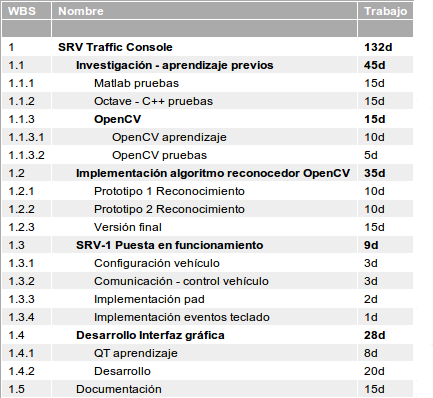
\includegraphics[width=6.5cm]{tareas-gantt.png}
\end{figure}

}

\frame{\frametitle{\textcolor{black}{Diagrama de Gantt}}

\begin{figure}[H]
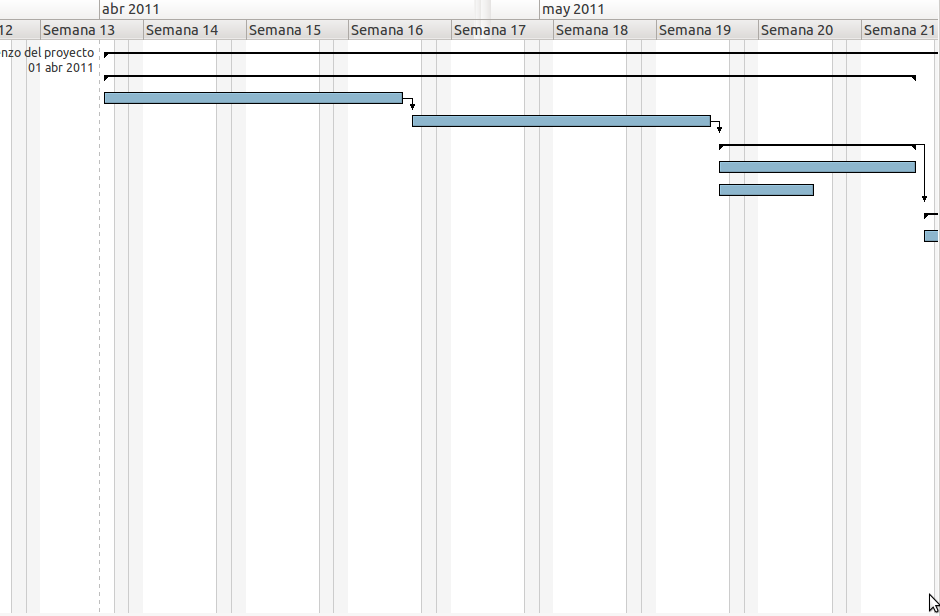
\includegraphics[width=4.4cm]{gantt-1.png}
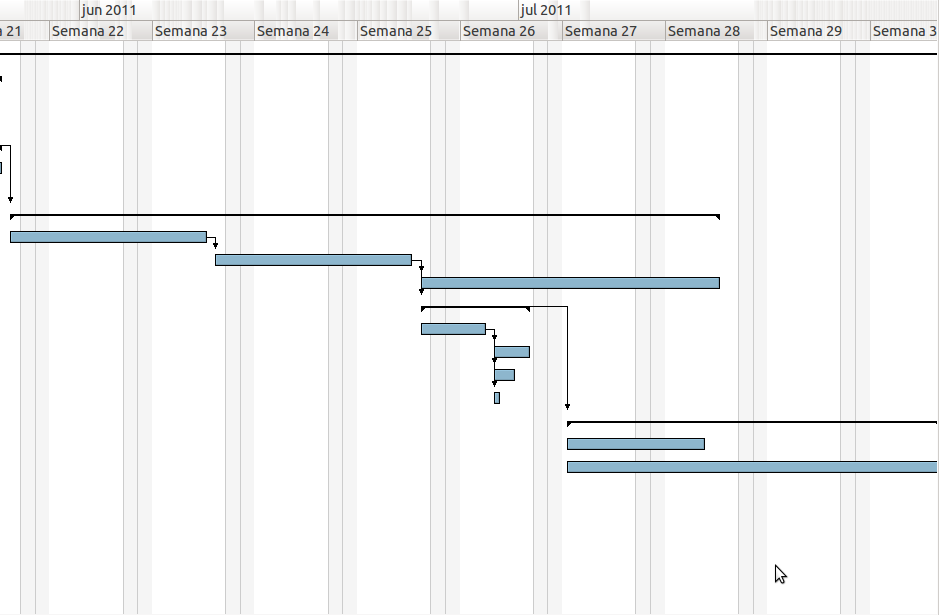
\includegraphics[width=4.4cm]{gantt-2.png}
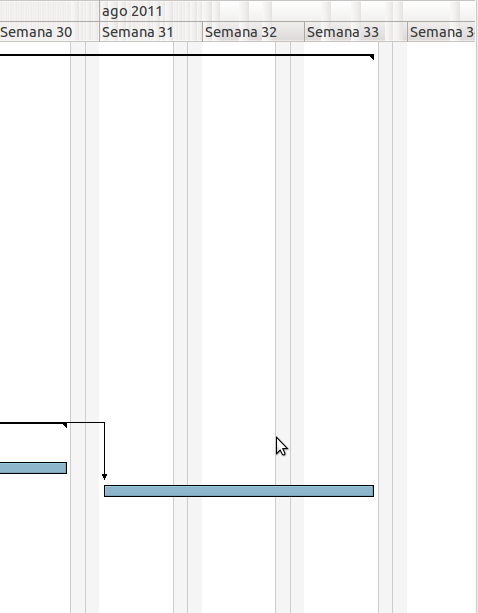
\includegraphics[width=2.25cm]{gantt-3.png}
\end{figure}

}



\section{Desarrollo}



\frame{\frametitle{\textcolor{black}{Comunicación}}

Las imágenes son captadas por el ordenador a partir de la cámara para su procesamiento.

\begin{figure}[H]
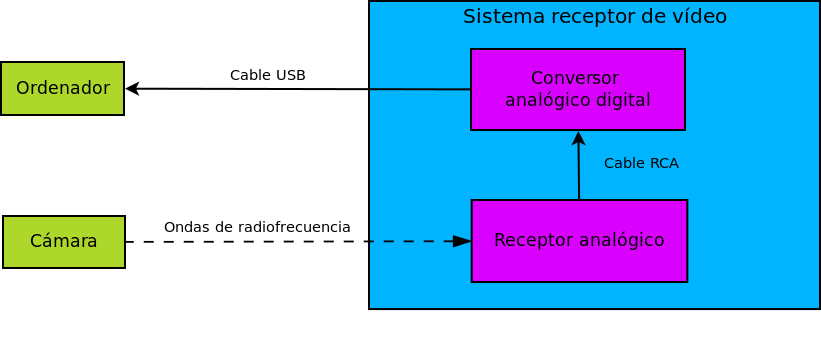
\includegraphics[width=7.5cm]{esquema-sistema-receptor-video.png}
\end{figure}

Una vez procesadas las imágenes se envía la respuesta al vehículo.

\begin{figure}[H]
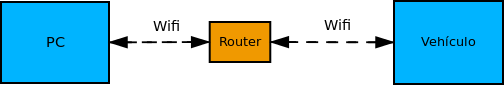
\includegraphics[width=7.5cm]{comunicacion-coche-robot.png}
\end{figure}

}


\frame{\frametitle{\textcolor{black}{Metodología de desarrollo}}

\begin{figure}[H]
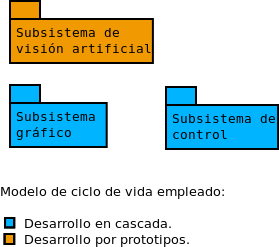
\includegraphics[width=6.5cm]{subsistemas.png}
\end{figure}

}




\section{Software de reconocimiento}

\subsection{Herramienta utilizada}

\frame{\frametitle{\textcolor{black}{OpenCV}}


El software de visión artificial ha sido elaborado haciendo uso de la biblioteca OpenCV para el lenguaje C. Esta biblioteca incluye los elementos necesarios para el tratamiento de imágenes para proporcionar al vehículo de un sistema de reconocimiento de señales de tráfico.

\begin{figure}[H]

\includegraphics[width=4.5cm]{opencv-logo.png}
\end{figure}

}

\subsection{Elementos reconocibles}

\frame{\frametitle{\textcolor{black}{Señales de tráfico}}

Las señales de tráfico detectables por el sistema son las siguientes:

\begin{figure}[H]
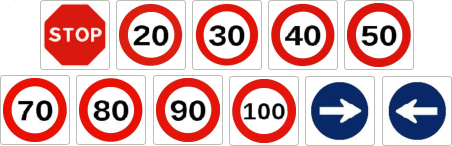
\includegraphics[width=7.5cm]{seniales.png}
\end{figure}

Entre las señales incluidas disponemos las diferentes señales indicadoras de velocidad máxima, existiendo desde la de 20 km/h hasta la de 100 km/h con el objetivo de poder ajustar automáticamente la velocidad del vehículo en función de la señal detectada.

Por otro lado existen las señales indicadoras de dirección obligatoria, con el fin de efectuar giros y la señal de stop con el propósito de efectuar paradas de manera automática.
}





\subsection{Prototipo 1}

\frame{\frametitle{\textcolor{black}{Paso 1: segmentación por color}}


\begin{itemize}

\item Como paso inicial se realizó una segmentación por color siguiendo el modelo tradicional RGB:
 
\begin{figure}[H]
  \begin{center}
      \begin{tabular}{cc p{7cm}p{7cm}}
        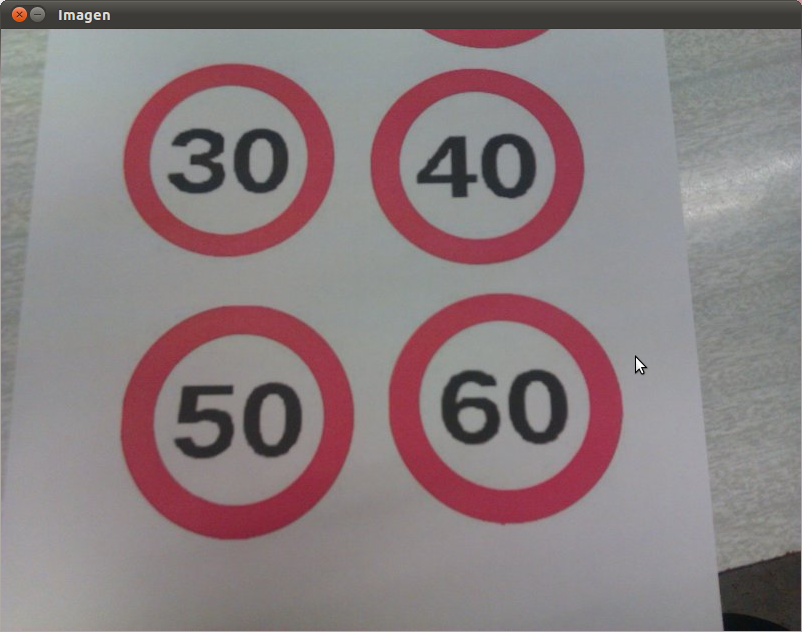
\includegraphics[width=4.5cm]{im-entrada.png} & 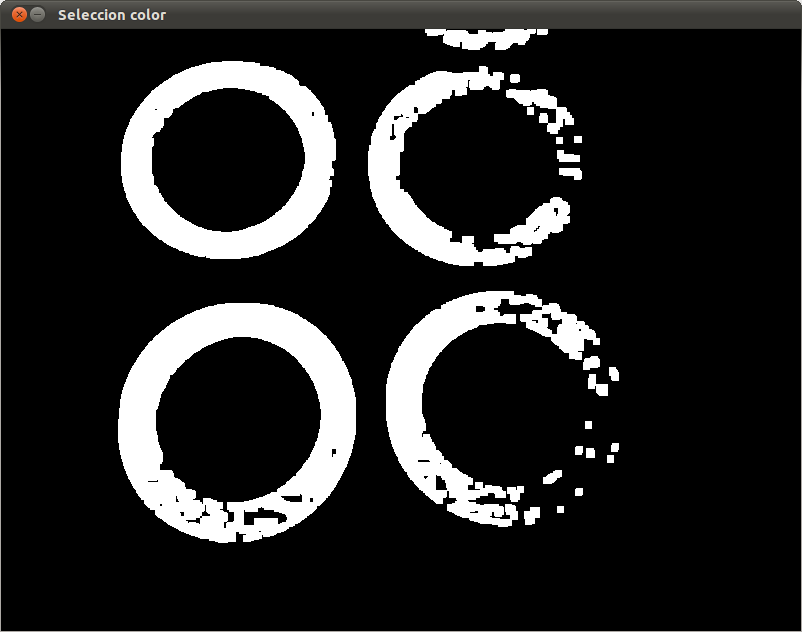
\includegraphics[width=4.5cm]{paso0.png}\\
        {Imagen de entrada (a).} & {Imagen resultante (b).}\\
      \end{tabular}
    \label{fig:ejemplo-selec-color}
  \end{center}
\end{figure}

\end{itemize}

}


\frame{\frametitle{\textcolor{black}{Paso 2: extraer objetos}}

\begin{itemize}

\item Posteriormente se establecen las regiones de interés:
 
\begin{figure}[H]
  \begin{center}
    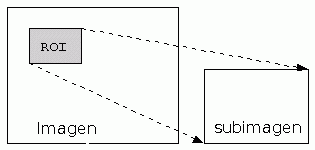
\includegraphics[scale=0.5]{roi.png}
  \end{center}
\end{figure}


\item Posteriormente se copia la imagen empleando una máscara:
 
\begin{figure}[H]
  \begin{center}
      \begin{tabular}{ccc p{3cm}p{3cm}p{3cm}}
        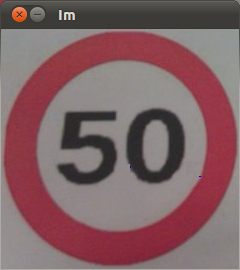
\includegraphics[width=1.8cm]{mascara1.png} &  
\includegraphics[width=1.8cm]{mascara2.png} & 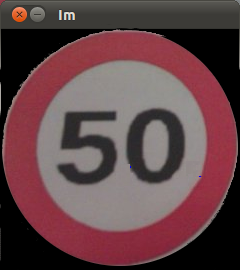
\includegraphics[width=1.8cm]{mascara3.png} \\
        {(\emph{a})} & {(\emph{b})} & {(\emph{c})} \\
      \end{tabular}
  \end{center}
\end{figure}


\end{itemize}

}

\frame{\frametitle{\textcolor{black}{Paso 3: clasificación}}

Para la clasificación se ha utilizado una técnica denominada Template Matching o Comparación de Plantillas:


\begin{figure}[H]
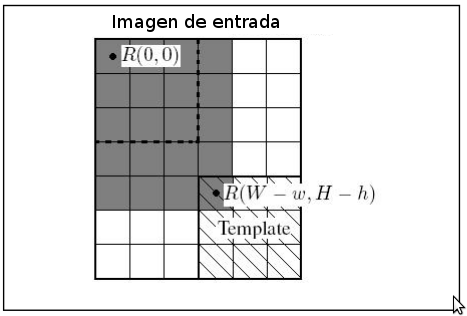
\includegraphics[width=7.5cm]{ejemplo-template.png}
\end{figure}


}


\frame{\frametitle{\textcolor{black}{Problemas detectados}}

Los problemas que han llevado a cabo el rechazo de este primer prototipo han sido los siguientes:

\begin{itemize}

\item  El problema de la utilización de una segmentación por color siguiendo el modelo RGB es que sufre una extrema sensibilidad de variación de los valores de un determinado color a las condiciones lumínicas del entorno. Esto ocasiona que el prototipo desarrollado solo sea funcional en un único entorno, por ejemplo, la sala donde se ha desarrollado y probado, dejando de ser funcional en otras situaciones y lugares siendo necesario idear una nueva metodología de segmentación para el siguiente prototipo.

\item El problema del Template Matching es que ha de comparar muchas características (para él, un píxel es una característica), y si tenemos en cuenta que en la base de datos encontramos N señales, observamos que con este método el resultado no ofrece garantías de funcionamiento en tiempo real, condición indispensable del proyecto.

\end{itemize}
}




\subsection{Prototipo 2}

\frame{\frametitle{\textcolor{black}{Reconocimiento de patrones}}

\begin{itemize}

\item Para este segundo prototipo se emplearon técnicas propias del reconocimiento de patrones.

\item Para poder clasificar satisfactoriamente los elementos, es necesario un proceso de aprendizaje previo en el cual el sistema crea un modelo de cada una de las clases a partir de una secuencia de entrenamiento o conjunto de vectores de características de cada una de las clases.

\item Debido a esta razón, debemos previamente, antes de realizar cualquier tarea de clasificación, elaborar un conjunto de vectores de características o también denominado matriz de modelos con el fin de cotejar las características del elemento a identificar con los datos de la matriz modelos. A la fase de obtención de la matriz de modelos se le denomina etapa de entrenamiento en un sistema de reconocimiento de patrones.

\item Al conjunto de características de una clase se denomina patrón. 

\end{itemize}
}


\frame{\frametitle{\textcolor{black}{Reconocimiento de patrones}}

\begin{itemize}
\item Antes de proceder con la extracción de los datos se realiza una segmentación por color, aunque en esta ocasión se ha realizado siguiendo el modelo de color HSV.

\item La aplicación de este modelo resulta mucho más ventajosa con respecto al modelo RGB debido a que HSV, (Matiz, Saturación, Valor) sólo precisa de un solo valor numérico para detectar el color, desde tonos relativamente ligeros hasta los tonos más oscuros centrándonos en el matiz y la saturación.

\item Entre los datos extraídos disponemos:

\begin{itemize}
\item Forma de la figura: círculo u octógono.
\item Perímetro del objeto/s interior/es.
\item Área del objeto/s interior/es.
\item Número de piezas interiores.
\item Número de vértices de las figuras interiores.
\end{itemize}


\end{itemize}

}

\frame{\frametitle{\textcolor{black}{Reconocimiento de patrones}}

Todos estos datos obtenidos durante la etapa de entrenamiento conforman un patrón, en la tabla se puede apreciar los diferentes datos obtenidos para algunas de las clases del sistema:\\

\begin{table}[H]
  \begin{center}
    \begin{tabular}{|p{2.5cm}|p{1cm}|p{1cm}|p{1cm}|p{1cm}|}
      \hline
        Señal:  & 
\includegraphics[width=1cm]{1.jpg} & 
\includegraphics[width=1cm]{2.jpg}  & 
\includegraphics[width=1cm]{3.jpg} & 
\includegraphics[width=1cm]{4.jpg} \\
      \hline

      Identificador: & 1 & 2 & 3 & 4 \\
      \hline
      Figura externa:& 8 & 9 & 9 & 9 \\     
      \hline
      Perímetro:& 506.877 & 1025.25 & 1565.18 & 1971.43 \\
      \hline 
      Área: & 8384.5 & 12774.5 & 17323.5 & 21771 \\ 
      \hline
      Número de vértices: & 39 & 77 & 125 & 156 \\ 
      \hline
      Piezas interiores: & 4 & 2 & 2 & 2 \\
      \hline
    \end{tabular}
  \end{center}
\end{table}

}

\frame{\frametitle{\textcolor{black}{Clasificación}}

Por tanto la matriz de modelos obtenida queda de la siguiente manera:\\

\[
 M =
 \begin{pmatrix}
  1 & 2 & 3 & 4 \\
  8 & 9 & 9 & 9 \\     
  506.877 & 1025.25 & 1565.18 & 1971.43 \\
  8384.5 & 12774.5 & 17323.5 & 21771 \\ 
  39 & 77 & 125 & 156 \\
  4 & 2 & 2 & 2 \\
 \end{pmatrix}
\]

Y el patrón del elemento a identificar:

    \[
    Vdesconocido =
    \begin{pmatrix}
      8\\     
      502.237 \\
      4022 \\ 
      34 \\
      4 
      \nocite{}
    \end{pmatrix}
    \]
}

\frame{\frametitle{\textcolor{black}{Vecino más cercano}}


\begin{figure}[H]
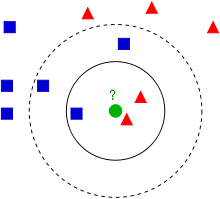
\includegraphics[width=3.5cm]{vecino.png}
\end{figure}

Se selecciona la clase correspondiente al elemento más cercano, las medidas son calculadas mediante la distancia euclídea. 

   \[
    d(x_{i},y_{j}) = \sqrt{\sum_{r=1}^p (x_{ir}-x_{jr})^2}
    \nocite{}
    \]
}


\frame{\frametitle{\textcolor{black}{Problemas detectados}}


Los problemas que han llevado a cabo el rechazo de este segundo prototipo han sido los siguientes:

\begin{itemize}

\item Los datos obtenidos durante la extracción de características tales como área, perímetro, número de vértices, número de objetos interiores de la señal, entre otros, no resultaban determinantes y excluyentes a la hora de realizar la clasificación proporcionando un alto número de errores cuando el objetivo es elaborar un sistema lo más fiable y eficiente posible.

\item Como punto positivo, se ha comprobado que el algoritmo del vecino más cercano presenta un funcionamiento más adecuado a las características exigibles del proyecto ya que proporciona una buena relación entre tiempo computacional y efectividad. Por otro lado, el algoritmo presenta la posibilidad de identificación de más de una clase.

\end{itemize}


}

\subsection{Prototipo 3}

\frame{\frametitle{\textcolor{black}{Extracción de características}}

Para el último prototipo se ha empleado la misma técnica de clasificación pero trabajando con diferentes datos en la matriz de modelos. La matriz de modelos contendrá la imagen de los elementos interiores de las señales de tráfico dispuestos en columnas. Posteriormente se aplica la misma clasificación con el algoritmo del vecino más cercano.

\begin{figure}[H]
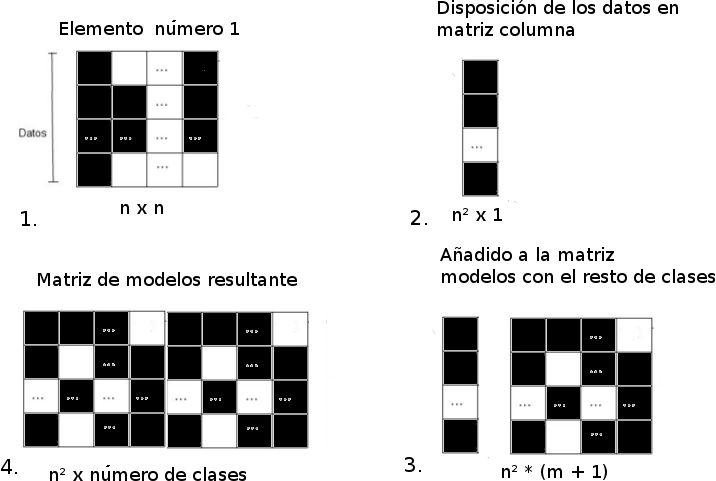
\includegraphics[width=7.5cm]{entrenamiento.png}
\end{figure}

}


\frame{\frametitle{\textcolor{black}{Clasificación}}


Para clasificar se realiza la llamada del algoritmo del vecino más cercano a cada objeto interno de la señal, en el caso mostrado son el número cero y el número cinco. Por tanto si dentro de un objeto circular de color rojo se localizan ambos elementos, determinaremos que se trata de una señal de 50 km/h.

\begin{figure}[H]
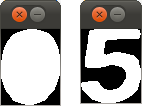
\includegraphics[width=1.5cm]{elementos.png}
\end{figure}

\begin{figure}[H]
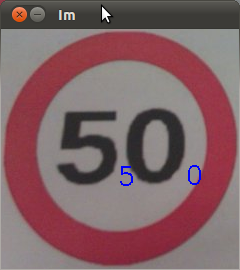
\includegraphics[width=1.5cm]{salida3.png}
\end{figure}

}



\section{Software de control}


\frame{\frametitle{\textcolor{black}{Surveyor Robot Software}}
Para el control del vehículo se ha utilizado un software denominado Surveyor Robot Software, el cual ha sido desarrollado por John Cummins junto con los agentes de laboratorio de la Universidad de Brooklyn con la asistencia de M.P. Azhar, y la supervisión del profesor Sklar empleando el lenguaje de programación C++.

El código ha sido ligeramente modificado para adaptarlo a las necesidades del proyecto.

\begin{figure}[H]
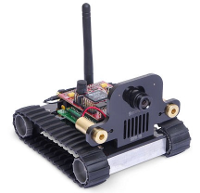
\includegraphics[width=3.5cm]{srv-1.png}
\end{figure}

}



\section{Interfaz}

\subsection{Herramienta}

\frame{\frametitle{\textcolor{black}{Qt}}

\begin{itemize}

\item Se consideró necesario proporcionar a la aplicación de una interfaz gráfica sencilla pero a la vez funcional teniendo como principal objetivo ofrecer al usuario, tras una visión rápida, la localización de los diferentes elementos para control del vehículo y deducir su funcionamiento.

\item La herramienta empleada ha sido una biblioteca multiplataforma específica para el desarrollo de aplicaciones con una interfaz gráfica de usuario, dicha biblioteca es Qt, la cual emplea el estándar C++.

\end{itemize}


\begin{figure}[H]

\includegraphics[width=2.5cm]{qt-logo.jpg}
\end{figure}

}

\subsection{Elementos incorporados}

\frame{\frametitle{\textcolor{black}{Interfaz}}

Los elementos incorporados en la ventana principal son los siguientes:

\begin{itemize}
\item Panel para el visionado de las imágenes captadas por la cámara.
\item Conjunto de botones para manejo del vehículo, con imágenes representativas de su acción.
\item Panel para el visionado de resultados donde se mostrarán aquellas señales de tráfico detectadas.
\item Información acerca del detector de distancias.
\end{itemize}


\begin{figure}[H]
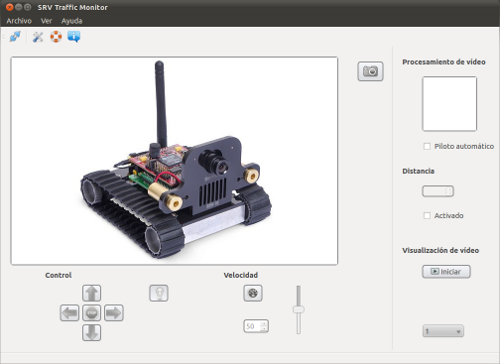
\includegraphics[width=4.5cm]{ventana-principal.png}
\end{figure}

}



\section{Conclusiones}

\frame{\frametitle{\textcolor{black}{Objetivos logrados}}

Durante la realización del proyecto \emph{OpenTSR: Vehículo reconocedor de señales de tráfico} como trabajo de fin de carrera, he conseguido profundizar mi conocimiento en los siguientes campos:

\begin{itemize}
\item Ampliación de conocimientos sobre \LaTeX.
\item Profundización sobre el lenguaje C y C++.
\item Aprendizaje sobre programación por eventos.
\item Diseño y creación de interfaces gráficas haciendo uso de la biblioteca Qt.
\item Estudio de técnicas aplicables al procesamiento de imágenes.
\item Estudio de técnicas y algoritmos propios del reconocimiento de patrones.
\end{itemize}
}



\section{Referencias}

\frame{\frametitle{\textcolor{black}{Referencias}}

\begin{thebibliography}{8} 
\beamertemplatebookbibitems 

\bibitem{1}\color{black}
Qt Reference Documentation
\url{http://doc.qt.nokia.com/4.7-snapshot/designer-manual.html}

\bibitem{2}\color{black}
Reference of OpenCV Language Library.
\url{http://docs.opencv.org/}

\bibitem{3}\color{black}
Surveyor Corporation. 
\url{http://www.surveyor.com/SRV_info.html}

\bibitem{4}\color{black}
Francisco Palomo Lozano. Inmaculada Medina Bulo. Gerardo Aburruzaga García.
\emph{Fundamentos de C++}. Servicio de Publicaciones de la Universidad de Cádiz,
2006.

\bibitem{5}\color{black}
Gerardo Aburruzaga García.\emph{Make. Un programa para controlar la recompilación}
\url{http://www.uca.es/softwarelibre/publicaciones/make.pdf}

\bibitem{6}\color{black}
Gary Bradski. Adrian Kaehler. \emph{Learning OpenCV Computer Vision with the OpenCV Library}. O’Reilly Media, 2008.

\bibitem{7}\color{black}
Ben Collins-Sussman. Brian W. Fitzpatrick. C. Michael Pilato. \emph{Control de versiones con Subversion}. O’Reilly Media, 2006.

\bibitem{8}\color{black}
\emph{Wikibooks. The Book of LaTeX.} \url{http://en.wikibooks.org/wiki/LaTeX}

\end{thebibliography} 
}


\frame{\frametitle{\textcolor{black}{Final}}
{
\begin{center}
\huge{¿Preguntas?}
\begin{figure}[H]
\href{http://ph03nyx.deviantart.com/}{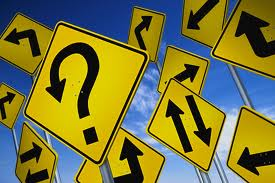
\includegraphics[width=2cm]{preguntas.jpg}}
\end{figure}
\end{center}

}
}

\end{document}
